El mundo es el entorno virtual donde los jugadores interactúan, exploran y se sumergen en la experiencia del juego. 
\textbf{Feed The Realm} cuenta con un sistema de creación de mundos que permite diseñar y construir entornos únicos y 
personalizados, que luego pueden ser publicados, compartidos con la comunidad y jugados por ella. Su valor agregado 
reside en las amplias opciones de personalización que ofrece para la creación de mundos.

\begin{figure}[H]
  \centering
  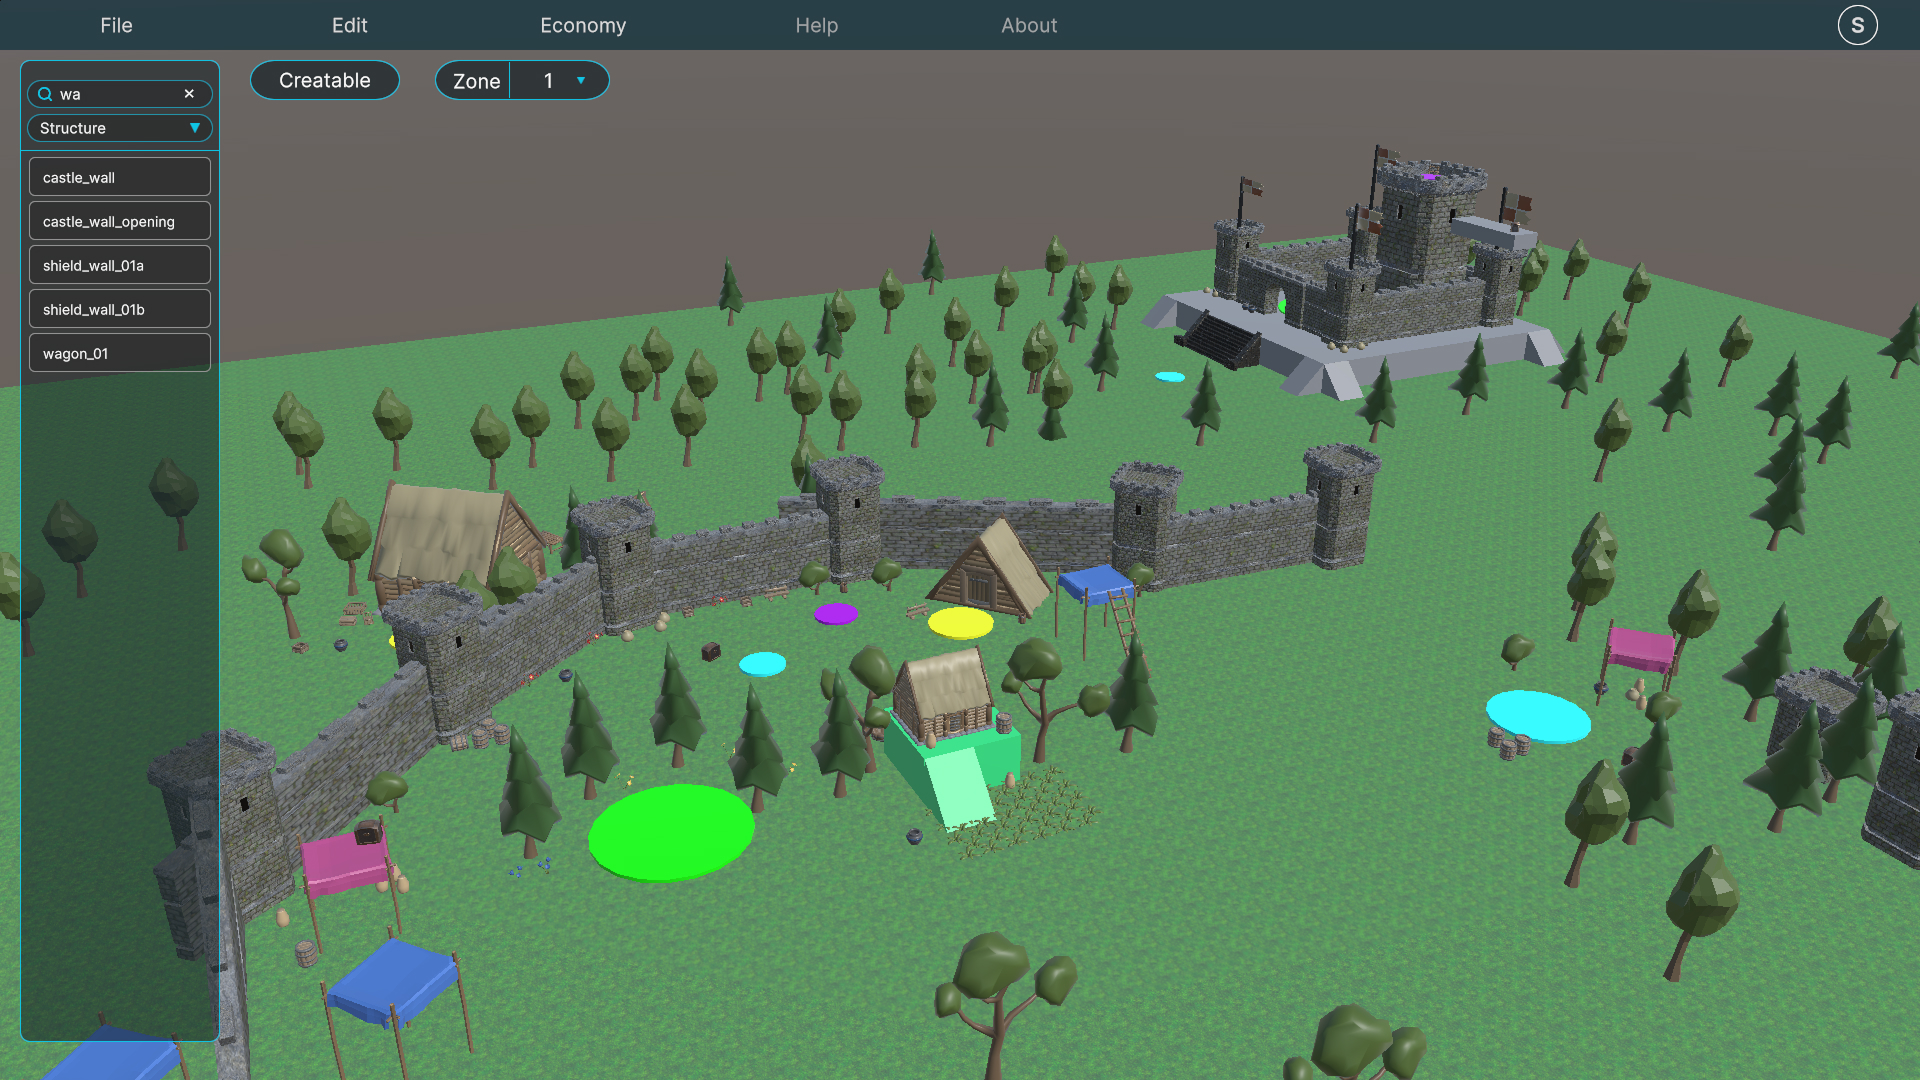
\includegraphics[width=\textwidth]{img/08-implemented-solution/product/custom-world.jpg}
  \caption{Captura de un mundo personalizado en el editor de mundos.}
  \label{fig:world-editor-example}
\end{figure}

\begin{figure}[H]
  \centering
  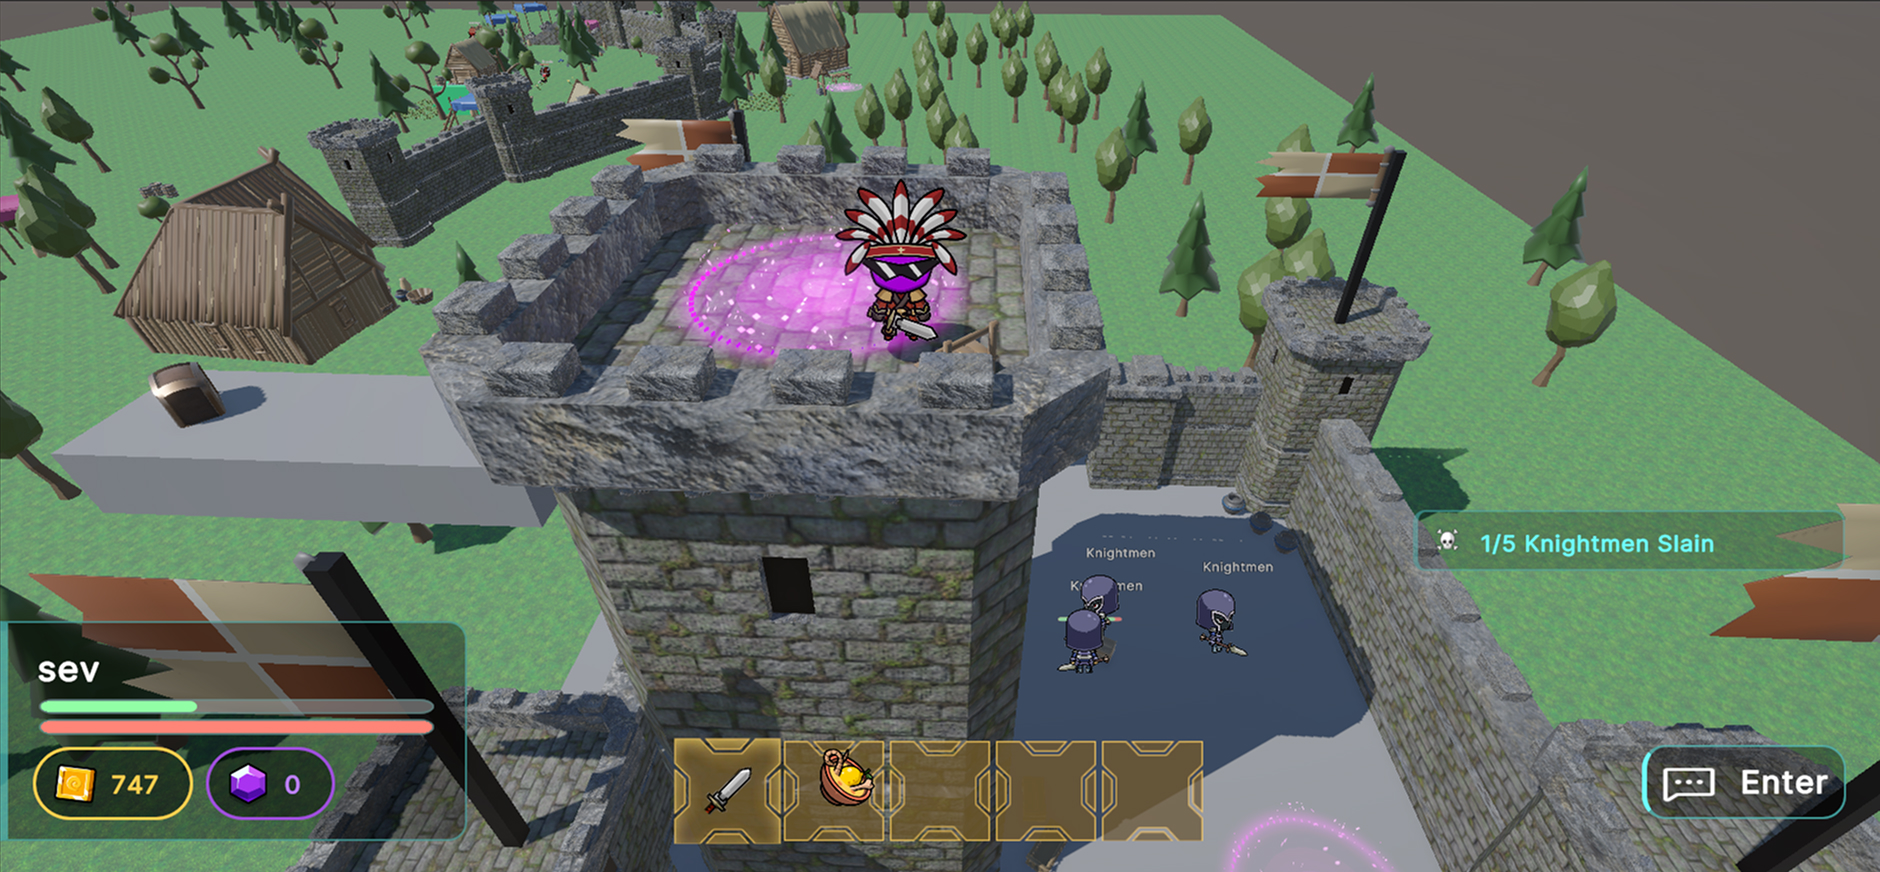
\includegraphics[width=\textwidth]{img/08-implemented-solution/product/player-on-tower.jpg}
  \caption{Captura de un Jugador en el mundo personalizado.}
  \label{fig:world-editor-example}
\end{figure}